\documentclass[fleqn]{article}
\usepackage{mathtools}
\usepackage{graphicx}
\usepackage{amssymb}
\usepackage[margin = 0.75in]{geometry}
\usepackage{enumerate}
\usepackage{color}
\usepackage{fancyvrb}
\usepackage{breqn}
\usepackage{fancyhdr}
\usepackage{multicol}
%\usepackage[latin1]{inputenc}
\usepackage{tikz}

\renewcommand{\thispagestyle}[1]{}
\pagestyle{fancy}
\lhead{\textbf{NAME:}}
\rhead{}

\begin{filecontents}{wolves.data}
1	4
2	15
3	22
4	26
5	41
6	55
7	46
8	42				
9	59
10	52
11	51
12	42
13	50
14	67
15	80
16	83
\end{filecontents}

\title{Exam 1 Modified}

\begin{document}
\title{Math 120R.002 Exam 1}
\author{Instructor: Ammon Washburn}
\date{10.02.15}
\maketitle

\section*{Instructions:} 
Please show all of your work for each question. Providing just the final answer \textbf{will not merit full credit}. The best way to ensure full credit is to provide the equation you use, show some work, and mark your final answer in an obvious way (circle, box, underline, etc.). The point values for each question are located at the beginning of the question.

\vspace{1in} 

\begin{tabular}{|p{6.5in}|} 
\hline 
\noindent By signing my name below, I agree that I am following all rules and regulations set forth by the Code of Academic Integrity.  Furthermore, I agree that I am following all rules set by my instructor and by the course policy for this exam.  This includes ensuring that all calculator programs except possibly QUADRATIC FORMULA have been deleted.\\
\vspace{.3 in}\\
\underline{Signature:	\hspace{2.5 in}	Date:\hspace{1.25 in}}\\
\hline 
\end{tabular} 

\pagebreak
\thispagestyle{fancy}{
\lhead{}
\rhead{/25}}

\section*{Free Response}

\begin{enumerate}
\item (15) For each part, decide whether or not the following could represent $y$ as a functions of $x$. If not, explain why not.
\begin{enumerate}
\item The graph of the curve provided.

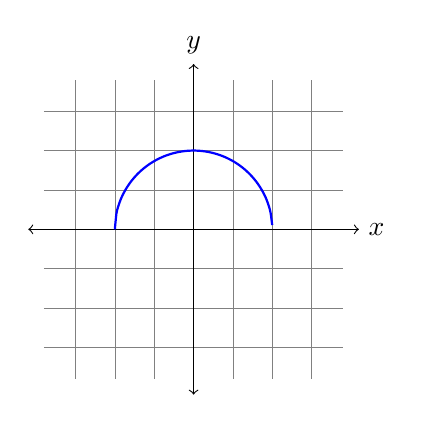
\begin{tikzpicture}
	\draw[very thin,color=gray,step=0.5] (-1.9,-1.9) grid (1.9,1.9);
	\draw[<->] (-2.1,0) -- (2.1,0) node[right] {$x$};
	\draw[<->] (0,-2.1) -- (0,2.1) node[above] {$y$};
	%\draw[<->] (0, -1) -- (2.6, 4.2) node[right] {$-2x_1 + x_2 \leq -1$};
	%\draw[<->] (0, 1) -- (3, -0.5) node[right] {$-x_1 + 2x_2 \leq -2$};
	%\draw plot (\x, {2*\x - 1}) node[right] {$-2x_1 + x_2 \leq -1$};
	%\draw plot (\x, {1 - 0.5*\x}) node[right] {$-x_1 + 2x_2 \leq -2$};
	\draw[thick,smooth,samples=100,domain=-1.0:1.0,-,color=blue] plot (\x, {pow(1-pow(\x,2),0.5});
    %\draw[thick,smooth,samples=100,domain=-1.0:1.0,-,color=blue] plot (\x, {-pow(1-pow(\x,2),0.5});
	%\draw[thick,smooth,samples=100,domain=0.0:2.0,->,color=blue] plot (\x, {-1.25*\x^0.33});
\end{tikzpicture}

\item $2y = 2xy - 7$
\vspace{0.5in}

\item 
\begin{tabular}{r|ccccc}
$x$ & 1 & 0 & 1 & 2 & 3 \\ \hline 
$y$ & 5 & 8 & 5 & 4 & 1 
\end{tabular}
\vspace{0.5in}

\item $y^6 - x^6  = 0$
\vspace{0.5in}

\item 
\begin{tabular}{r|ccccc}
$x$ & -1 & 0 & 1 & 2 & 3 \\ \hline 
$y$ & 1 & 1 & 2 & 2 & 3 
\end{tabular}
\vspace{0.5in}

\end{enumerate}

\item (5) Consider the functions $f(x) = 2x + 3$ and $g(x) = 7x + 8$. Find $h(x) = f(x)/g(x)$ and its domain.
\vspace{1in}

\item (5) Let $t(x) = \frac{2x-1}{x+3}$. Verify that $t(x)$ is one-to-one and find $t^{-1}(y)$.
\vspace{2in}

\pagebreak
\thispagestyle{fancy}{
\lhead{}
\rhead{/10}}

\item (10) The graph provided shows the population of wolves in Arizona and New Mexico due to the Mexican wolf blue range reintroduction project.

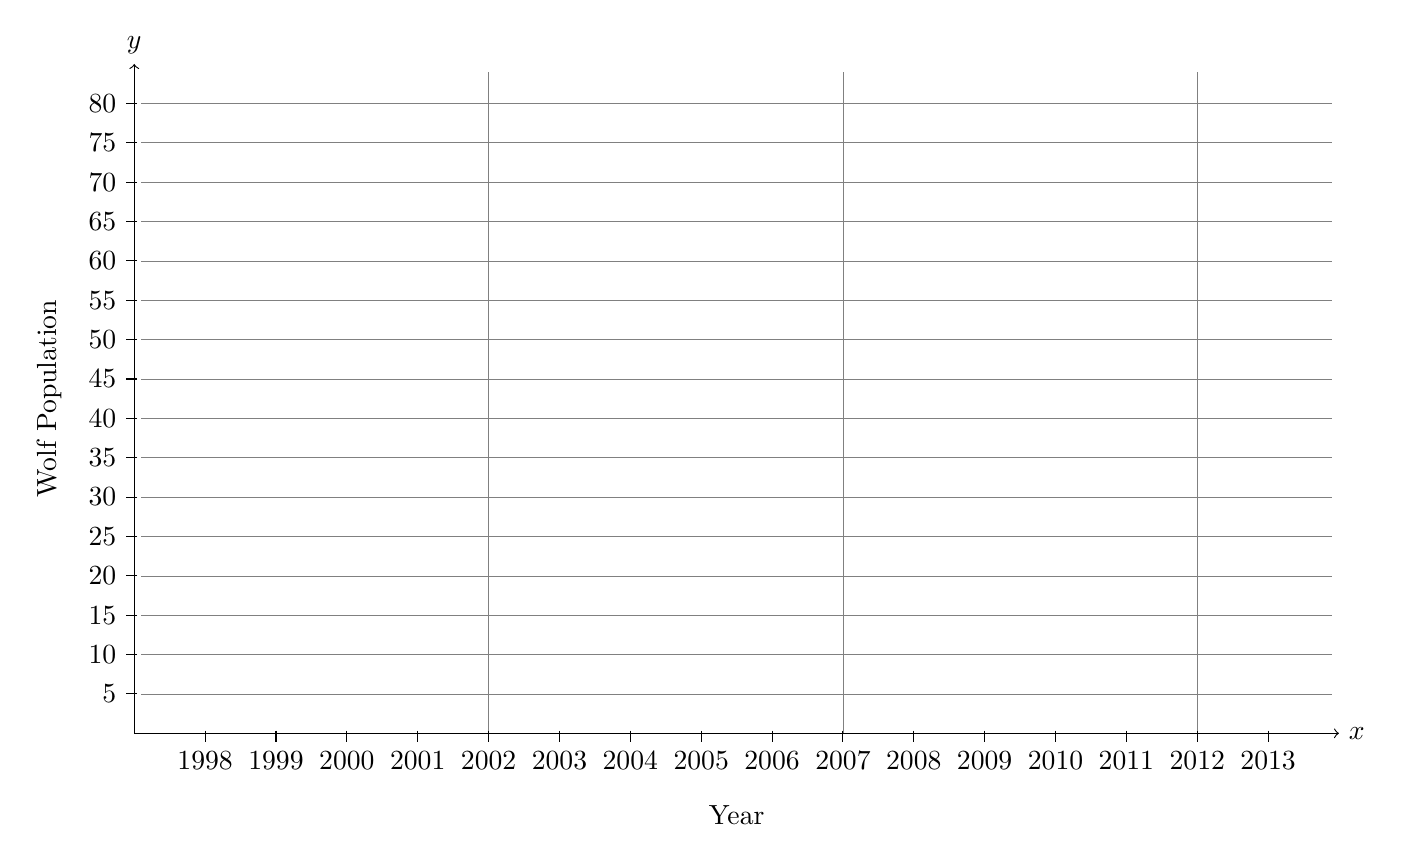
\begin{tikzpicture}[y=0.1cm, x=0.9cm]
\draw[very thin,color=gray,step=5] (0.1,0.1) grid (16.9,84);
\draw[->] (0, 0) -- coordinate (x axis mid) (17, 0) node[right] {$x$};
\draw[->] (0, 0) -- coordinate (y axis mid) (0, 85) node[above] {$y$};
\foreach \x in {1998,...,2013}
	\draw (\x-1997, 1pt) -- (\x-1997, -3pt) node[anchor=north] {\x};
\foreach \y in {5, 10,...,80}
	\draw (1pt, \y) -- (-3pt, \y) node[anchor=east] {\y};
\draw plot[mark=*] file {wolves.data};

\node[below=0.8cm] at (x axis mid) {Year};
\node[rotate=90, above=0.8cm] at (y axis mid) {Wolf Population};
\end{tikzpicture}

\begin{enumerate}
\item What is the average rate of change from 2001 to 2010? From 2003 to 2008? Provide units.
\vspace{1.5in}

\item What is/are the local minimum(s) of the wolf population? Provide year and number of wolves
\vspace{1in}

\end{enumerate}

\pagebreak
\thispagestyle{fancy}{
\lhead{}
\rhead{/35}}

\item (15) The relationship between the cost of shipping in dollars, $S$, and the number of pounds, $p$, at a local post office is given by 
\begin{align*}
T(p) &= \begin{cases}
15  & \qquad 0 \leq p \leq 5 \\
15 + 3(p - 5) & \qquad 5 < p \leq 25 \\
75 + 6(p - 25) & \qquad 25 < p \leq 70
\end{cases}
\end{align*}
\begin{enumerate}

\item If the cost of mailing a box was \$18, how many pounds did the box weigh?
\vspace{1in}

\item What is the domain of this function and the practical interpretation of the right end point?
\vspace{1in}

\item What are the practical interpretations of the slopes?
\vspace{0.75in}

\end{enumerate}

\item (20) Consider the function $g(x) = 1 - 3 \sqrt{x + 4}$.
\begin{enumerate}
\item What is the base function? What kinds of transformations are taking place (in order)?
\vspace{2in}

\item What is the domain of $g(x)$?

\vspace{1in}

\pagebreak
\thispagestyle{fancy}{
\lhead{}
\rhead{/15}}

\item Use the axes provided to plot $g(x) = 1 - 3 \sqrt{x + 4}$. 

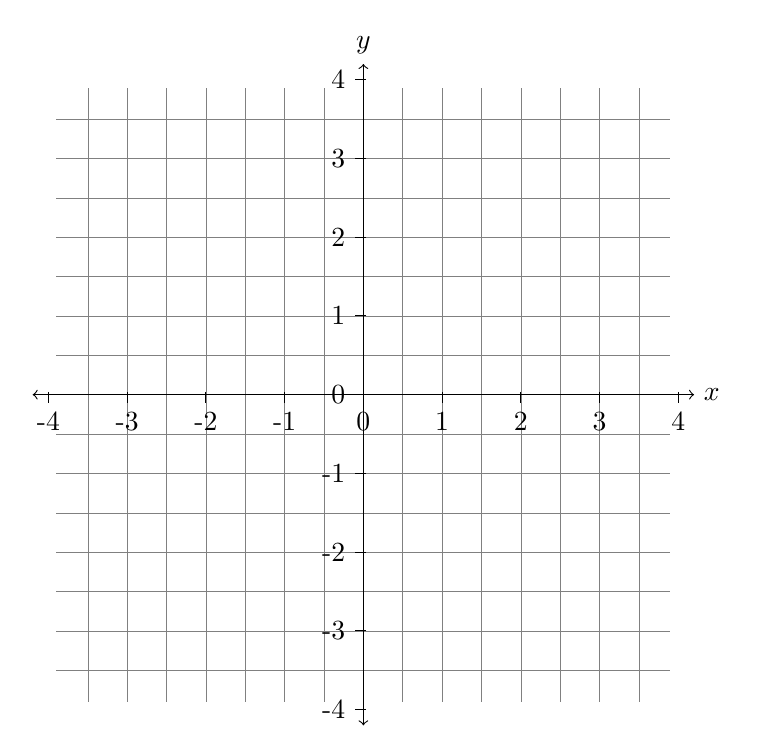
\begin{tikzpicture}
	\draw[very thin,color=gray,step=0.5] (-3.9,-3.9) grid (3.9,3.9);
	\draw[<->] (-4.2,0) -- (4.2,0) node[right] {$x$};
	\draw[<->] (0,-4.2) -- (0,4.2) node[above] {$y$};
\foreach \x in {-4, ..., 4}
	\draw (\x, 1pt) -- (\x, -3pt) node[anchor=north] {\x};
\foreach \y in {-4, ..., 4}
	\draw (1pt, \y) -- (-3pt, \y) node[anchor=east] {\y};
\end{tikzpicture}

\end{enumerate}

\section*{Multiple Choice}

\item (5) Find the domain of the function $\displaystyle f(x) = \frac{\sqrt[]{1-x}}{x+5}$.
\begin{multicols}{3}
\begin{enumerate}[(a)\,]
\item $(-\infty,-5) \cup (-5,1]$
\item $(-\infty, 1) \cup (1, 5]$ 
\item $[1,5) \cup (5,\infty)$
\item $(-\infty, \infty)$
\item $(1,\infty]$
\end{enumerate}
\end{multicols}

\vspace{1in}

\item (5) Is the function $f(x) = \frac{x^2}{x^2+1}$ even, odd, or neither?
\begin{multicols}{3}
\begin{enumerate}[(a)\,]
\item even
\item odd
\item neither
\end{enumerate}
\end{multicols}

\vspace{1in}

\item (5) Let $t(x) = \frac{1}{x-1}$ and $r(x) = \frac{x-3}{x}$. What is the domain of $(t \circ r)(x)$?
\begin{multicols}{3}
\begin{enumerate}
\item $(-\infty,0)$
\item $(-\infty,\infty)$
\item $(-\infty,1) \cup (1,\infty)$
\item $(-\infty,0) \cup (0,\infty)$
\item $(-\infty,0) \cup (0,1) \cup (1,\infty)$
\end{enumerate}

\end{multicols}

\pagebreak
\thispagestyle{fancy}{
\lhead{}
\rhead{/15}
\rfoot{/100}}

\item (5) On what intervals is the function increasing and the function decreasing?

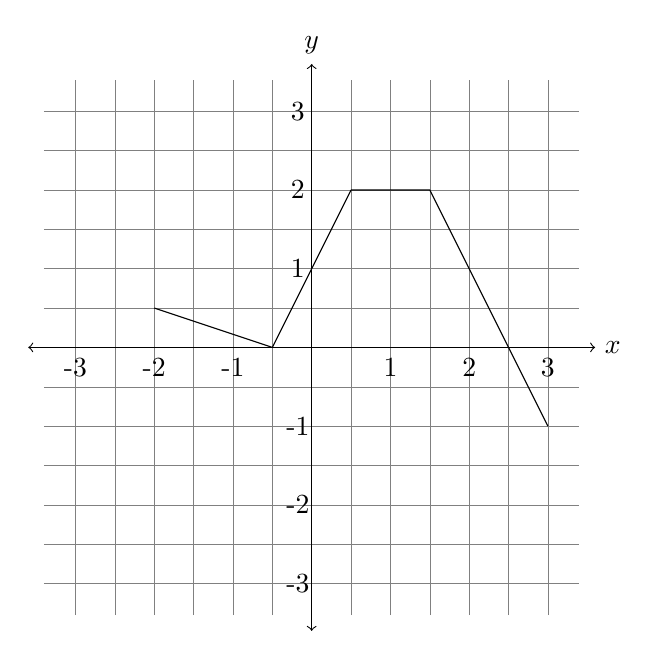
\begin{tikzpicture}
	\draw[very thin,color=gray,step=0.5] (-3.4,-3.4) grid (3.4,3.4);
	\draw[<->] (-3.6,0) -- (3.6,0) node[right] {$x$};
	\draw[<->] (0,-3.6) -- (0,3.6) node[above] {$y$};
    \draw (-2,.5) -- (-.5,0) -- (.5,2);
    \draw (.5,2) -- (1.5,2) -- (3,-1);
	%\draw[<->] (0, -1) -- (2.6, 4.2) node[right] {$-2x_1 + x_2 \leq -1$};
	%\draw[<->] (0, 1) -- (3, -0.5) node[right] {$-x_1 + 2x_2 \leq -2$};
	%\draw plot (\x, {2*\x - 1}) node[right] {$-2x_1 + x_2 \leq -1$};
	%\draw plot (\x, {1 - 0.5*\x}) node[right] {$-x_1 + 2x_2 \leq -2$};
    \node at (1,-0.25) {1};
    \node at (2,-.25) {2};
    \node at (-1,-.25) {-1};
    \node at (-2,-.25) {-2};
    \node at (3,-0.25) {3};
    \node at (-3,-.25) {-3};
    \node at (-.175,1) {1};
    \node at (-.175,2) {2};
    \node at (-.175,-1) {-1};
    \node at (-.175,-2) {-2};
    \node at (-.175,3) {3};
    \node at (-.175,-3) {-3};
	%\draw[thick,smooth,samples=100,domain=0.0:2.0,->,color=blue] plot (\x, {-1.25*\x^0.33});
\end{tikzpicture}


\begin{enumerate}
\item Increasing: $(-2,-0.5)\cup(1.5,3)$ ~ Decreasing: $(-0.5,0.5)$
\item Increasing: $(2.5,3)$ ~ Decreasing: $(-2,-0.5)\cup(-0.5,2.5)$
\item Increasing: $(-0.5,0.5)$ ~ Decreasing: $(-2,-0.5)\cup(1.5,3)$
\item Increasing: $(-2,0.5)$ ~ Decreasing: $(0.5,3)$
\item Increasing: $(-0.5,1.5)$ ~ Decreasing: $(1.5,3)$
\end{enumerate}

\item (5) Determine the equation in point slope form that passes through the point $(a,b)$ and is perpendicular to the line $y=-4x+6$

\begin{multicols}{3}
\begin{enumerate}
\item $y=-4(x-a)+b$
\item $y=4(x-a)+b$
\item $y = \frac{1}{4}(x+a) +b$
\item $y=\frac{1}{4}(x-a) +b$
\item $y=-\frac{1}{4}(x-a)+b$
\end{enumerate}
\end{multicols}

\item (5) Suppose the ordered pair (3,4) is on the graph of $y=g(x)$. What ordered pair must be on the graph of $y=g(\frac{1}{3}x)+2$?

\begin{multicols}{3}
\begin{enumerate}
\item $(1,12)$
\item $(1,6)$
\item $(6,6)$
\item $(9,2)$
\item $(9,6)$
\end{enumerate}
\end{multicols}




% \item (5) Which of the following statements are true? 
% \begin{multicols}{2}
% \begin{enumerate}[I.]
% \item $ \sqrt{x^2 + 64} = x + 8 $
% \item $3x^{-1} = \displaystyle \frac{1}{3x}$
% \end{enumerate}
% \end{multicols}

% \begin{multicols}{4}
% \begin{enumerate}[(a)\,]
% \item Both statements are true
% \item Only statement I. is true
% \item Only statement II. is true
% \item Neither statement is true
% \end{enumerate}
% \end{multicols}

% \pagebreak
% \thispagestyle{fancy}{
% \lhead{}
% \rhead{/10}
% \rfoot{/100}}

% \item (5) The graph of the entire function if given. 
% What is its range?

% \begin{tikzpicture}[y=0.5cm, x=2cm]
% 	\draw[very thin,color=gray,step=0.5] (-3.1,-7.9) grid (2.1,9.9);
% 	\draw[<->] (-3.2,0) -- (2.2,0) node[right] {$x$};
% 	\draw[<->] (0,-8.2) -- (0,10.2) node[above] {$y$};
% 	\draw[thick,smooth,samples=100,domain=-3.0:2.0,color=blue] plot (\x, {\x^3 - 5*\x + 5});

% \foreach \x in {-3, -2, -1, 1, 2}
% 	\draw (\x, 1pt) -- (\x, -3pt) node[anchor=north] {\x};
% \foreach \y in {-8, -6,...,10}
% 	\draw (1pt, \y) -- (-3pt, \y) node[anchor=east] {\y};
% \draw plot[mark=*, mark options={fill=blue, draw=blue}, mark size=3pt] (2, 3);
% \draw plot[mark=*, mark options={fill=white, draw=blue}, mark size=3pt] (-3, -7);
% \end{tikzpicture}
% \begin{multicols}{3}
% \begin{enumerate}[(a)\,]
% \item $(-7, 9.25]$
% \item $(-3, 2]$
% \item $(-7, 3]$
% \item $(-3, 9.25]$
% \item $[-7, 3)$
% \end{enumerate}
% \end{multicols}


\vspace{2in}
\end{enumerate}

\end{document}